\chapter{ПРОГРАМНИЙ МОДУЛЬ ВИЗНАЧЕННЯ МЕТРИК ЦІЛЬОВОЇ ПРОГРАМИ ДЛЯ ПІДВИЩЕННЯ ЕФЕКТИВНОСТІ ДОСЛІДЖЕННЯ ЇЇ ПОТЕНЦІЙНО-НЕБЕЗПЕЧНИХ ДЕФЕКТІВ}
\label{3section::doc}\label{3section:id1}

\section{Структурна схема алгоритму та основні функціональні елементи}
\label{3section:id2}
Підчас аналізу предметної області мною була запропонована структурна схема програмно-технічного комплексу виявлення залежностей між метриками інтегрованих властивостей програм.
\begin{figure} [h]
    \centering
    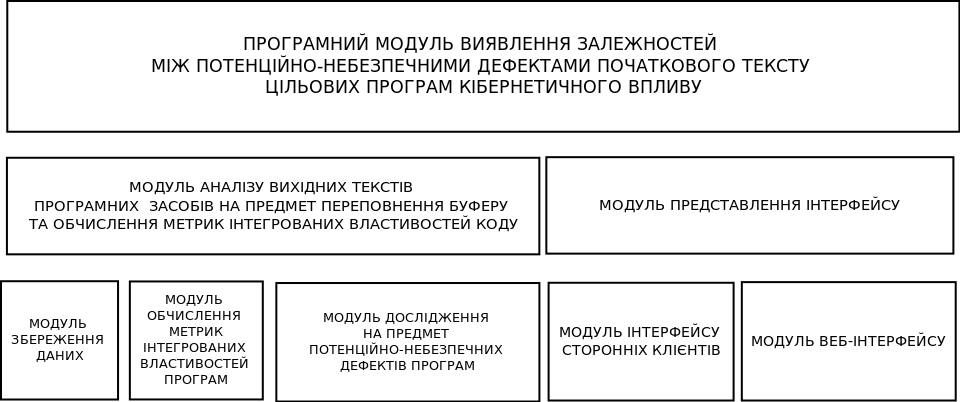
\includegraphics[width=16cm]{general_structure.png}
    \caption{Структурна схема модулю визначення метрик цільової програми}
    \label{fig:general_structure}
\end{figure}
(Рис \,\ref{fig:general_structure})

Модулі програмно-технічного комплексу:
\begin{enumerate}
 \item Модуль аналізу вихідних текстів програмних засобів на предмет переповнення буферу та обчислення метрик інтегрованих властивостей коду;
 \item Модуль представлення інтерфейсу.
\end{enumerate}

Модуль аналізу вихідних текстів програмних засобів включає в себе декілька підмодулів:
\begin{itemize}
 \item Модуль обчислення метрик інтегрованих властивостей програм;
 \item Модуль досліджнення на предмет потенційно-небезпечних дефектів програм;
 \item Модуль збереження даних.
\end{itemize}

В свою чергу, модуль представлення інтерфейсу містить 2 підмодулі:
\begin{itemize}
 \item Модуль веб-інтерфейсу
 \item Модуль інтерфейсу сторонніх клієнтів
\end{itemize}

\subsubsection{Модуль аналізу вихідних текстів програмних засобів}
\label{module_analize}
Даний модуль реалізує аналіз метричних характеристик досліджуваних програм та потенційно-небезпечних дефектів реакції програм, та на основі цих даних робить кількісну оцінку вразливих участків коду. Дані характеристики зберігаються в БД (SQLite)

\subsubsection{Модуль обчислення метрик інтегрованих властивостей програм}
\label{module_metrix_calculations}

\subsubsection{Модуль досліджнення на предмет потенційно-небезпечних дефектів програм}
\label{module_vulnurabilities_search}

\subsubsection{Модуль збереження даних}
\label{module_data_storing}

\subsubsection{Модуль представлення інтерфейсу}
\label{module_interface}

\subsubsection{Модуль веб-інтерфейсу}
\label{module_web_interface}

\subsubsection{Модуль інтерфейсу сторонніх клієнтів}
\label{module_endpoints}

\section{Інтерфейс користувача}
\label{3section:id3}

\section{Керівництво щодо розгортання та експлуатації}
\label{3section:id4}

\section*{Висновки}
\addcontentsline{toc}{section}{Висновки}
Отже,
